%************************************************
\chapter{\texttt{aRNAque}: An evolutionary algorithm for inverse folding inspired by Lévy flights.}\label{ch:arnaque}

	A Lévy flight is a random walk with step sizes that follow a heavy-tailed probability distribution. This type of random walk, with many small steps and a few large ones, has inspired many applications in genetic programming and evolutionary algorithms in recent years, but is yet to be applied to RNA design. Here we study the inverse folding problem for RNA, viz. the discovery of sequences that fold into given target secondary structures. We implement a Lévy mutation scheme in an updated version of \texttt{aRNAque}, an evolutionary inverse folding algorithm, and apply it to the design of RNAs with and without pseudoknots. We find that the Lévy mutation scheme increases the diversity of designed RNA sequences and reduces the average number of evaluations of the evolutionary algorithm. The results show improved performance on both \texttt{Pseudobase++} and the \texttt{Eterna100} datasets, outperforming existing inverse folding tools. We propose that a Lévy flight offers a better standard mutation scheme for optimizing RNA design.
	
	We provide in this work an updated version of \texttt{aRNAque} supporting pseudoknotted RNA target structures. In addition to the  support for pseudoknots, we provide an updated mutation mode based on a Zipf distribution. For a given population of RNA sequences, an exponent $c$ of the Zipf distribution, and the mutation parameters: $P_N$ and $P_C$, we present the mutation algorithm in Algorithm \ref{Algo:Lévy}.
	
\section{Material and methods}

\subsection{Inverse folding evolutionary algorithm (EA)}
Below, we provide a brief overview of our evolutionary search algorithm and our mutation scheme. 
In general, an evolutionary search algorithm on any fitness landscape consists of three main parts, which in the context of RNA inverse folding are as follows: %(Figure \ref{Fig:model}):
\begin{itemize}
	\item Initialization: generating a random initial population of RNA sequences compatible with the given target secondary structure.
	\item Evaluation and selection: evaluating a population of RNA sequences consists of two steps: 1) fold each sequence into a secondary structure and assign it a weight based on its similarity to the target structure. 2) select a weighted random sample with replacement from the current population to generate a new population. A detailed description of the objective function used in \texttt{aRNAque} is provided in \cite{merleau2021simple}. 
	\item Mutation (or move) operation: define a set of rules or steps used to produce new sequences from the selected or initial ones. This component is elaborated further in the next subsection.
	
\end{itemize}
%\begin{figure}[H]
%    \centering
%    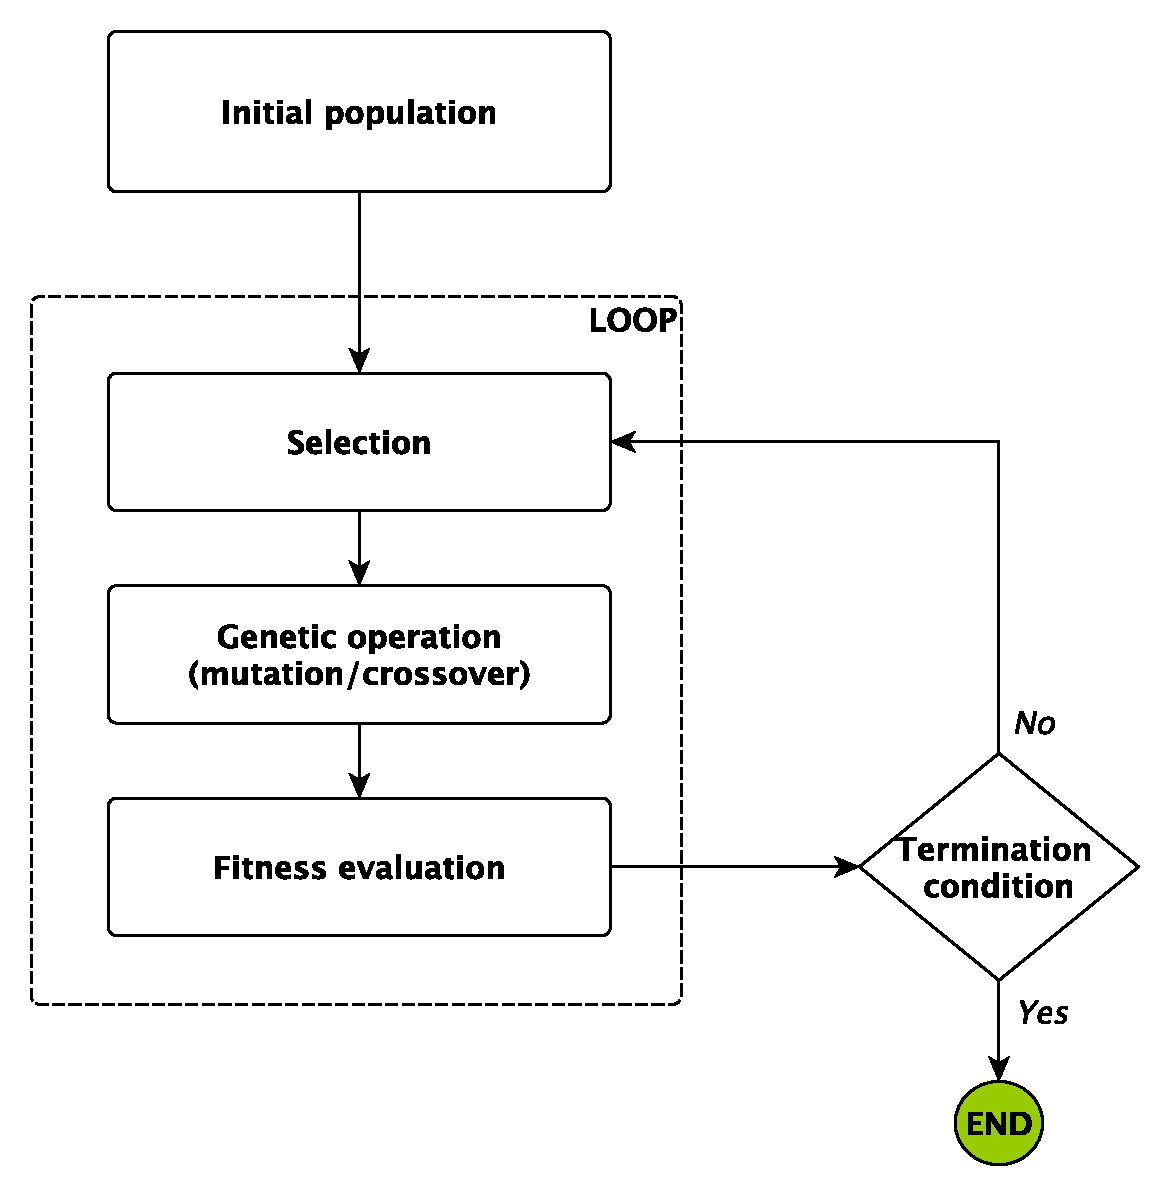
\includegraphics[width=0.5\textwidth]{figures/EA_draw.pdf}
%    \caption{Evolutionary algorithm flow diagram}
%    \label{Fig:model}
%\end{figure}


\subsection*{Mutation mode}
For a given target RNA secondary structure $\sigma*$ of length $L$, the space of potential solutions to the inverse folding problem is $S=\{A,C,G,U\}^L$.
An evolutionary algorithm explores the space $S$ through its move (or mutation) operator.
\begin{figure}[t!]
	\centering
	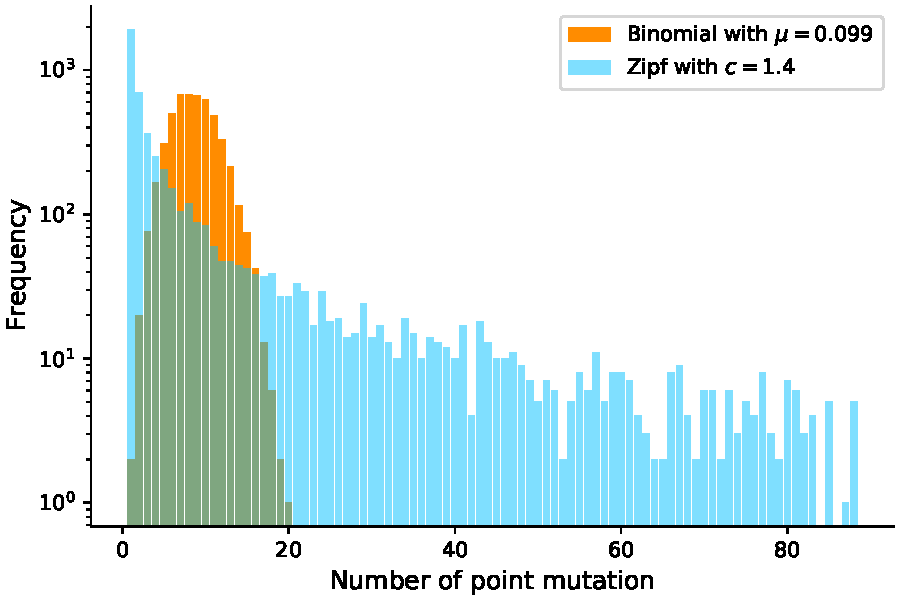
\includegraphics[width=1.0 \linewidth]{../res/images/arnaque/bino_zipf.pdf}
	\caption{$5000$ samplings Binomial and Zipf distributions. Both distributions have a mean of $8.7$ point mutations for a sequence of length $88$ nucleotides.}\label{Fig:histomut}
\end{figure}
Given a sequence $\phi \in S$, a sequence $\phi' \in S$ is said to be an $n$-point mutation of $\phi$ if it differs from $\phi$ at $n$ nucleotides; i.e. $h(\phi, \phi')=n$ where $h(.,.)$ is the hamming distance on $S$. 

A mutation mode is a random variable $U$ taking values in $\{1,...,L\}$. $P(U=n)$ is defined as the probability that, exactly $n$ nucleotides, selected uniformly at random undergo point mutation during a mutation event. $U$ can generally be any probability distribution. We examined the binomial and Zipf distributions:

\begin{itemize}
	\item Binomial mutation: here $U$ has a binomial distribution: 
	$$
	P(U=n)= \binom{l}{n} \mu^n (1-\mu)^{l-n}
	$$
	for some $0 \leq \mu \leq 1$, such that $u=\mu \cdot l$. We can think of this mutation mode arising from each nucleotide of an RNA sequence independently undergoing a point mutation with probability $\mu$, i.e. $\mu$ is the per-nucleotide or point mutation rate. 
	
	\item Lévy mutation: $U$ has a Zipf distribution given by: 
	$$
	P(U=n)= \frac{1/n^c}{ \sum_{k=1}^{l}{1/k^c}}
	$$
	where $c>0$ is the value of the exponent characterizing the distribution.
\end{itemize}

\begin{figure}[t!]
	\centering
	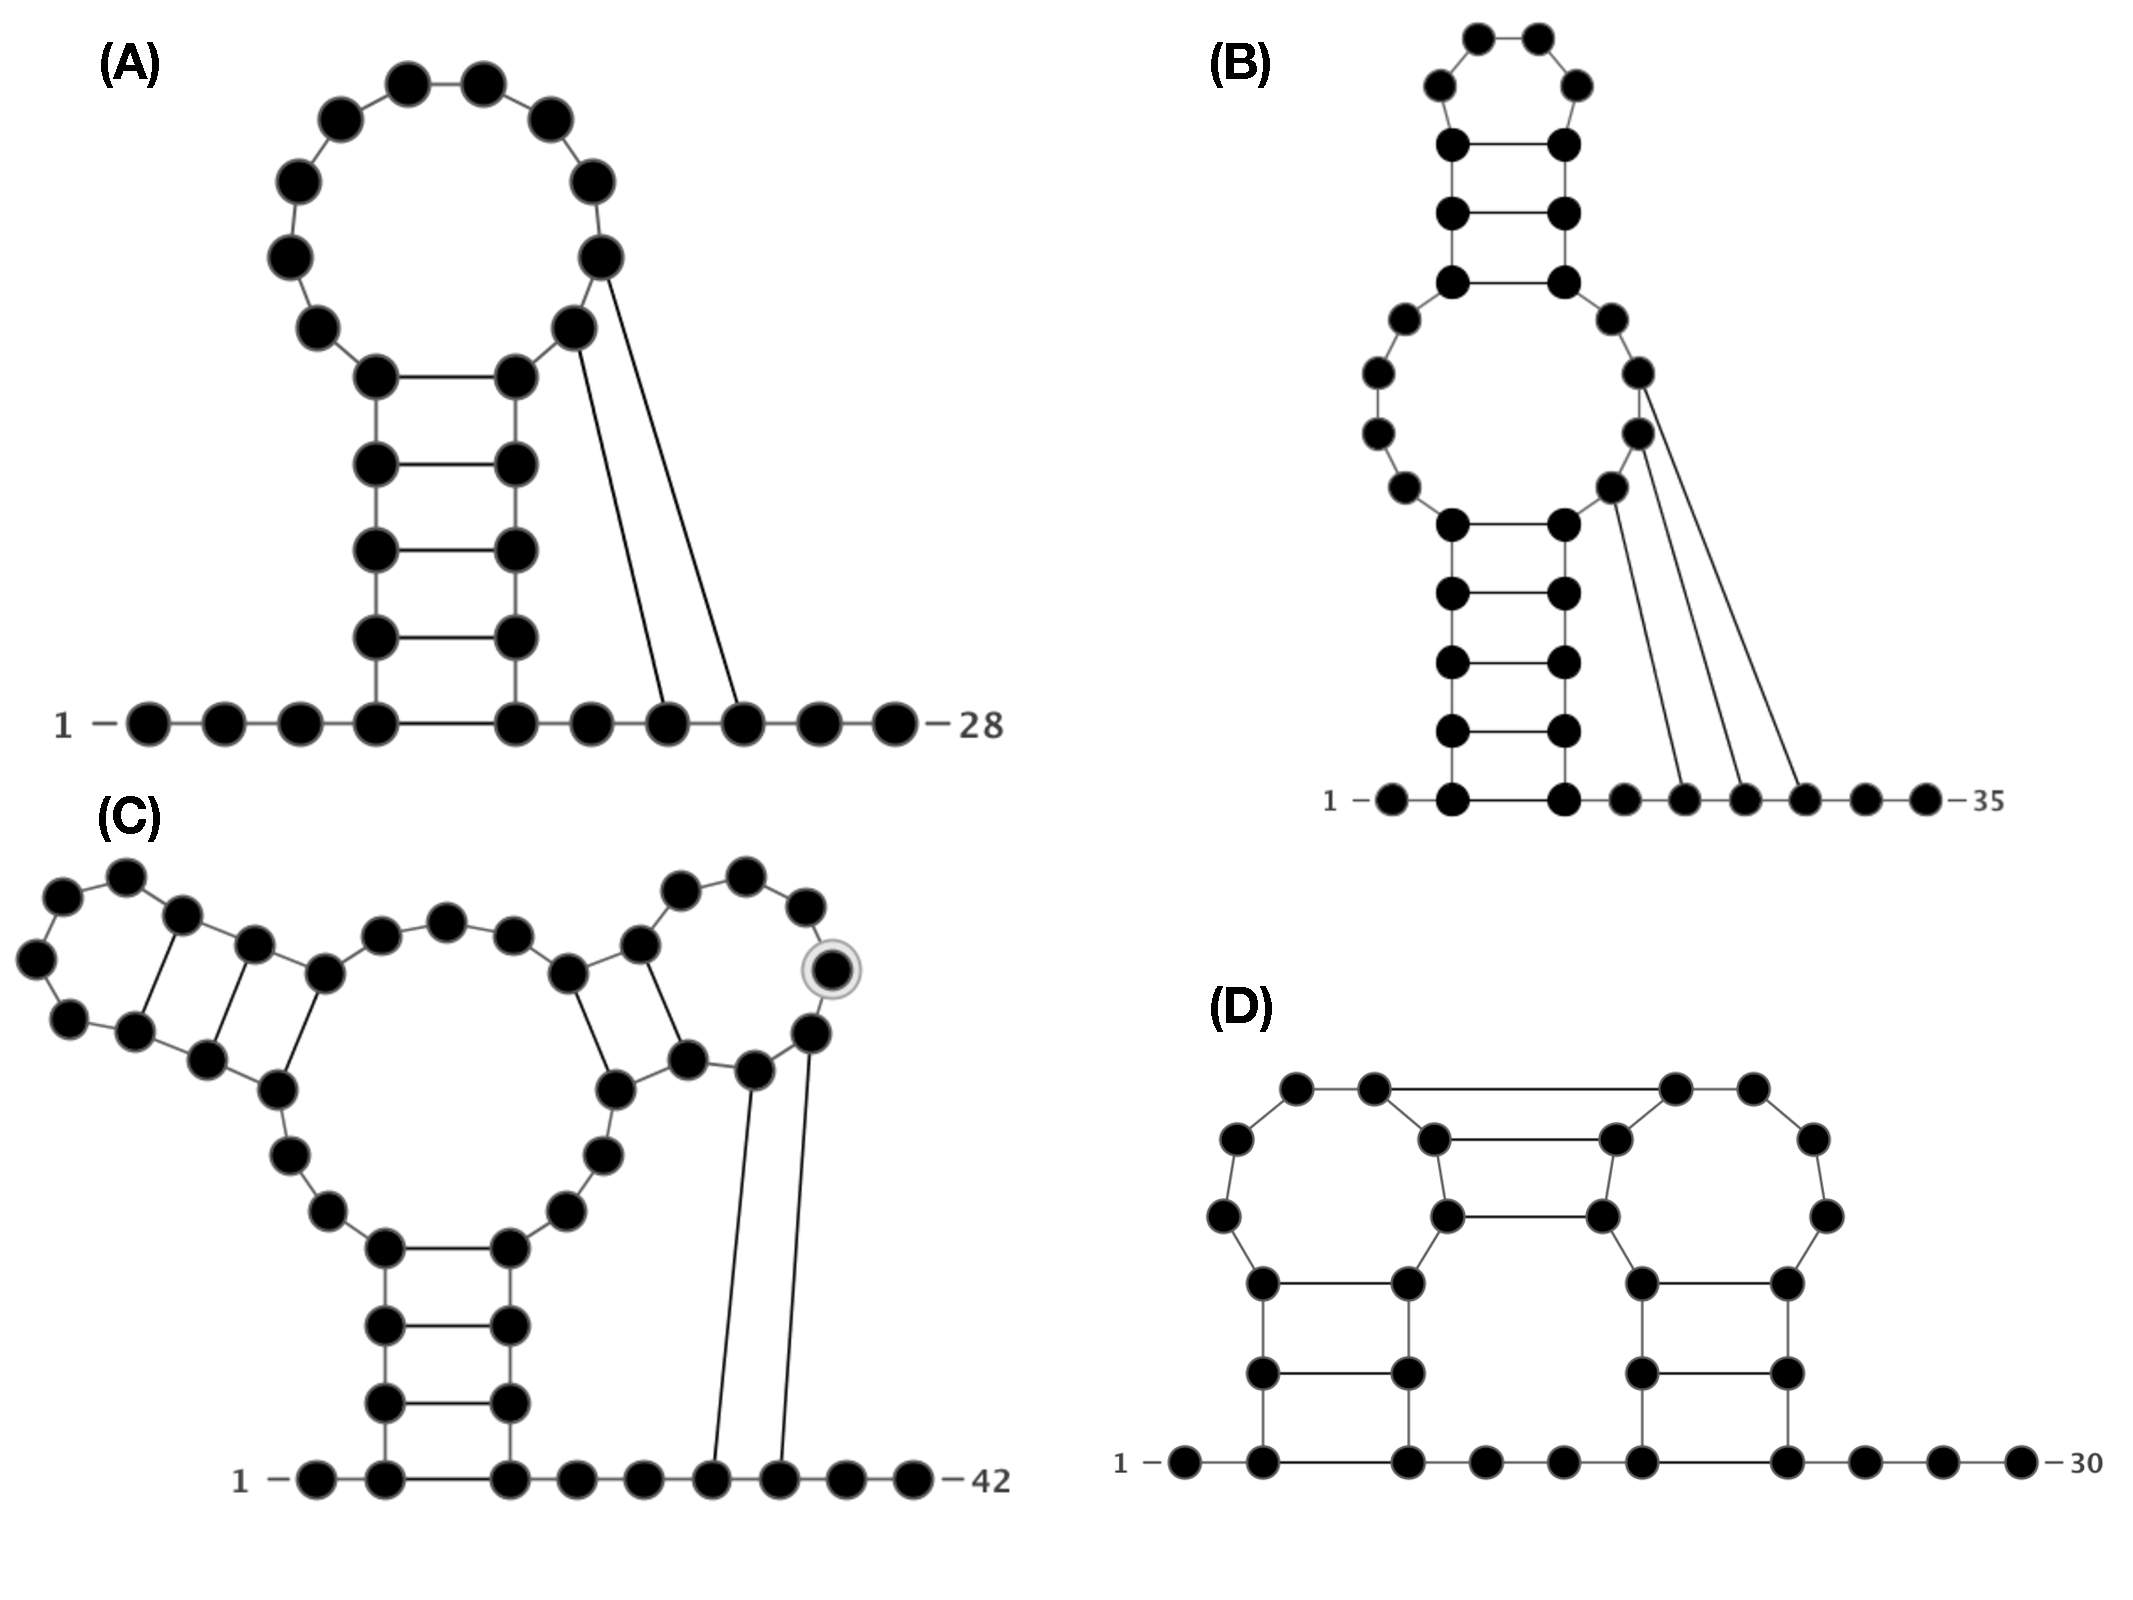
\includegraphics[width=1.0 \linewidth]{../res/images/arnaque/pk_type.pdf}
	\caption{Types of pseudoknots accommodated by aRNAque. (A) Hairpin (H-type) pseudoknot. (B) Bulge (B-type) pseudoknot. (C) Complex hairpin (cH-type) pseudoknot. (D) Kissing hairpin  (K-type) pseudoknot.\label{Fig:pk_type}}
	
\end{figure}
Figure \ref{Fig:histomut} Figure 3 shows the distribution of the number of point mutations on a sequence of length $88$ nucleotides for both mutation schemes. Both distributions have the same mean, and the difference between the two distributions is more perceptible on their tails. 

In the rest of this work, a local mutation will refer to a binomial mutation with parameter $\mu \approx 1/L$.


\begin{algorithm}[b!]
	\tcc{$P'=\{S'_1\dots S'_n\}$: the mutated population\; 
		$P= \{S_1\dots S_n\}$: a list of $n$ RNA sequences to mutate\;
		$P_{C}=\{w_{AU},w_{GU},w_{GC}\}$: a vector containing the weights associated with each canonical base pairs\;
		$P_{N}=\{w_{A},w_{U},w_{C}, w_{G}\}$: a vector containing the weights associated with each nucleotide\;
		$\mathcal{D}$: a given probability distribution (Lévy or Binomial) with parameter $p$ and $L$ where $L$ is the length of the target RNA structure}
	\KwInput{$P$, $\mathcal{D}(p, L)$, $P_{C}$,  $P_{N}$}
	\KwOutput{$P'$} 
	$ \{B_i\} \sim \mathcal{D}(p,L)$, where $i\in \{1,2,\dots,n\}$ \tcp*{Draw $n$ random numbers that follows a given distribution $\mathcal{D} (p,L)$ (Lévy or Binomial). $B_i$ is the number base pairs to mutate}
	$\{U_i\} \sim \mathcal{D}(p,L)$, where $i\in \{1,2,\dots,n\}$ \tcp*{Draw $n$ random numbers that follows the same distribution as $B_i$ (Lévy or Binomial). $U_i$ is the number non base pair positions to mutate}
	
	\For{ $i \in \{1, 2, \dots, n\}$ }{
		$S'\leftarrow P_i$ \tcp*{Assign the sequence $S_i \in P$ to $S'$ }
		\For{ $j \in \{1,2,...U_i\}$}{
			$r \in \{1,2,\dots, L\} \sim \mathcal{U}$ \tcp*{select uniformly a random position in the RNA sequence $S'$}
			$n_j \in \{A,U,C,G\} \sim P_N$ \tcp*{select a random nucleotide $n_j$ with respect to $P_N$} 
			$S'_r \leftarrow n_{j}$ \tcp*{replace the nucleotide at position $j$ in the RNA sequence $S'$ with $n_j$}
		}
		\For{ $j \in \{1,2,...B_i\}$}{
			$k_j \in \{AU,UA,CG,GC,GU,UG\} \sim P_C$ \tcp*{select a random base pair $k_{i}$ with respect to $P_C$}
			$b \in \{(b_1,b_2)_i\} \sim \mathcal{U}$ \tcp*{select uniformly a random pair of base pair positions}
			$S'_b \leftarrow k_{j}$ \tcp*{replace respectively the nucleotides at the base pair position $b_i \in b$ by $k \in k_j$}
			
		}
		$P' \gets P'\cup S'$ \tcp*{Add $S'$ to the list $P'$}
	}
	\caption{Mutation algorithm}\label{Algo:Lévy}
\end{algorithm}

%In addition to the two main features mentioned above, we also provide a web-server integrating an enriching interface to compare and analyse the designed sequences.

%%%%%%%%%%%%%%%%%%%%%%%%%%%%%%%%%%%%%%%%%%%%%%
%%                                          %%
%% Backmatter begins here                   %%
%%                                          %%
%%%%%%%%%%%%%%%%%%%%%%%%%%%%%%%%%%%%%%%%%%%%%%

\subsection{Parameter analysis and benchmark}
Here we analyse mutation parameters and compare local and Lévy mutation modes. 

\subsubsection{Benchmark data used}
To compare our new version of \texttt{aRNAque} with existing tools in the literature, we used the \texttt{PseudoBase++} benchmark datasets for  pseudoknotted target structures and the \texttt{Eterna100} dataset for pseudoknot-free target structures.

The \texttt{PseudoBase++} is a set of $265$ pseudoknotted RNA structures used to benchmark \texttt{Modena}. It was initially $304$ RNA secondary structures, but we excluded $37$ because they had non-canonical base pairs. We then grouped the structures into four pseudoknot motifs (Figure \ref{Fig:pk_type}): $209$ hairpin pseudoknots (H), $29$ bulge pseudoknots (B), $8$ complex hairpin pseudoknots (cH) and $4$ kissing hairpin pseudoknots (K).  

The~\(\texttt{Eterna100}\) dataset \cite{Eterna} is available in two versions and both contain a set of \(100\) target structures extracted from the \texttt{EteRNA} puzzle game and classified by their degree of difficulty. The \texttt{Eterna100-V1} was initially designed using \texttt{ViennaRNA} 1.8.5, which relies on Turner1999 energy parameters \cite{Turn1999}. Out of the $100$ targets secondary structures, $19$ turned out to be unsolvable using the recent version of \texttt{ViennaRNA} (Version $2.14$). Subsequently, an \texttt{Eterna100-V2} \cite{Eterna} was released in which the $19$ targets were slightly modified to be solvable using \texttt{ViennaRNA 2.14}. 

\subsection{Benchmark protocol}
\begin{figure*}[t!]
	\centering
	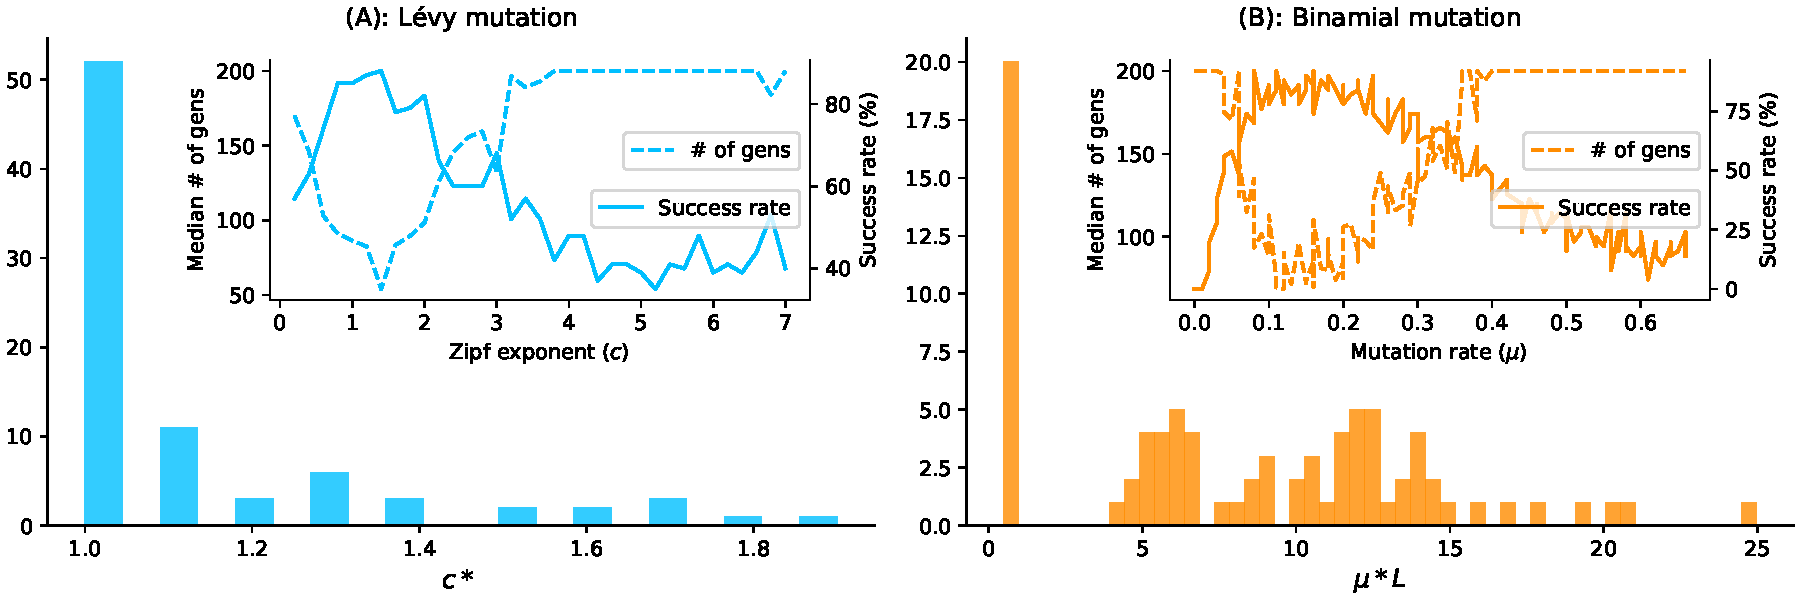
\includegraphics[width=1.0\linewidth]{../res/images/arnaque/Tuning.pdf}
	\caption{Parameter tuning for both binomial and Levy mutation schemes.(A) Lévy-flight parameter tuning. Histogram of best exponent parameter ($c*$) for a set of $81$ target structures with different pseudoknot patterns and various lengths. The most frequent best exponent value is $1$. Note that this corresponds to an exponent near 0 for the complementary cumulative distribution function. The inset figure shows the median generations and the success percentage \emph{vs.} the exponent parameter ($c$) for one of the pseudoknotted target of length $88$ with a broader range of $c$ (from $0$ to $7$ with a step size of $0.1$). (B) Binomial parameter tuning. Histogram of best mutation rate ($\mu^*$) for the same set of $81$ target structures with different pseudoknots and various lengths. The most frequent best parameter is the low mutation rate ($\approx 1/L$). For some structures, the mutation rate seems to be the high one for different lengths as well. Similar to the Levy mutation, The inset figure shows the median generations and the percentage of success \emph{vs.} the mutation rate ($\mu$) for one of the pseudoknotte} \label{Fig:tunning}
	\medskip
	\small.
\end{figure*}
The best mutation parameters obtained for both binomial and Lévy mutation modes are used to benchmark and compare the results on the entire datasets of RNA structures ($265$ from \texttt{PseudoBase++} and $100$ from \texttt{EteRNA100}). First, for each of the $365$ target structures $\sigma^*$ in the datasets, $20$ sequences were designed. To measure the performance of each tool, each designed sequence $s$ is folded into a secondary structure $\sigma$ and the similarities between $\sigma$ and $\sigma^*$ are computed using the base pair distance. Second, for each of the \texttt{Eterna100} target structures and a maximum of $5000$ generations (i.e. $50,000$ evaluations), $5$ to $20$ runs were launched independently, which results in at least $5$ designed sequences per target. We define success rate simply as the number of successfully designed targets. A target is considered successfully designed when at least one of the designed sequence folds into the target structure (i.e. the Hamming distance between the target structure and the MFE structure is $0$).

\subsubsection{Folding tools}
Two tools for pseudoknotted RNA folding are considered in this work: \texttt{HotKnots} and \texttt{IPknot}. For pseudoknot-free RNA folding, we used \texttt{RNAfold}.
For the mutation parameter analysis presented here, we used \texttt{IPknot}, and both \texttt{HotKnots} and \texttt{IPknot} for pseudoknotted targets. Furthermore, we considered \texttt{pkiss}, a well know tool for K-type pseudoknot prediction, but since the \texttt{PseudoBase++} dataset contains just $5$ K-type pseudoknotted structures and \texttt{pKiss} has higher time complexity ($O(n^6)$), we did not find it efficient for the benchmark we performed here. 
\subsubsection{Mutation parameters tuning}
One of the main challenges for an evolutionary algorithm is to find optimum parameters such as mutation rate, population size and selection function.
We used $81$ pseudoknotted targets with lengths from $25$ to $181$ nucleotides for the mutation parameter analysis. We set the maximum number of generations to $200$ and the population size to $100$. The best Lévy mutation parameter $c*$ (respectively $\mu*$ for the binomial mutation) has the lowest median number of generations. 

\begin{itemize}
	\item Binomial mutation: First, for each $\mu \in [0,1]$ with a step size of $0.005$, $50$ sequences were designed using \texttt{aRNAque} and the input pseudoknotted target structure was \texttt{PKB00342}. In Figure \ref{Fig:tunning}B, the inset figure shows the median number of generations and the success rate for each parameter $\mu$. The best mutation rate is $\mu*=0.085$ (with a median number of generation $93.5$ and a success rate of $92\%$). The critical range was identified to be from $0$ to $0.2$ and as $\mu$ becomes greater than $0.1$, the success rate decreases and the average number of generations increases. Second, for the $80$ target structures with pseudoknots, $20$ sequences were designed for $\mu \in [0,0.2]$ with a step size of $1/L$. Figure \ref{Fig:tunning}B shows the histogram of the best mutation rate found for each target structure. Two main regimes are visible: one regime in which the best mutation rate is the low one ($\approx 1/L$) and the second regime for which for which the high mutation rate was optimal. 
	
	%\begin{figure}[t!]
	%\centering
	%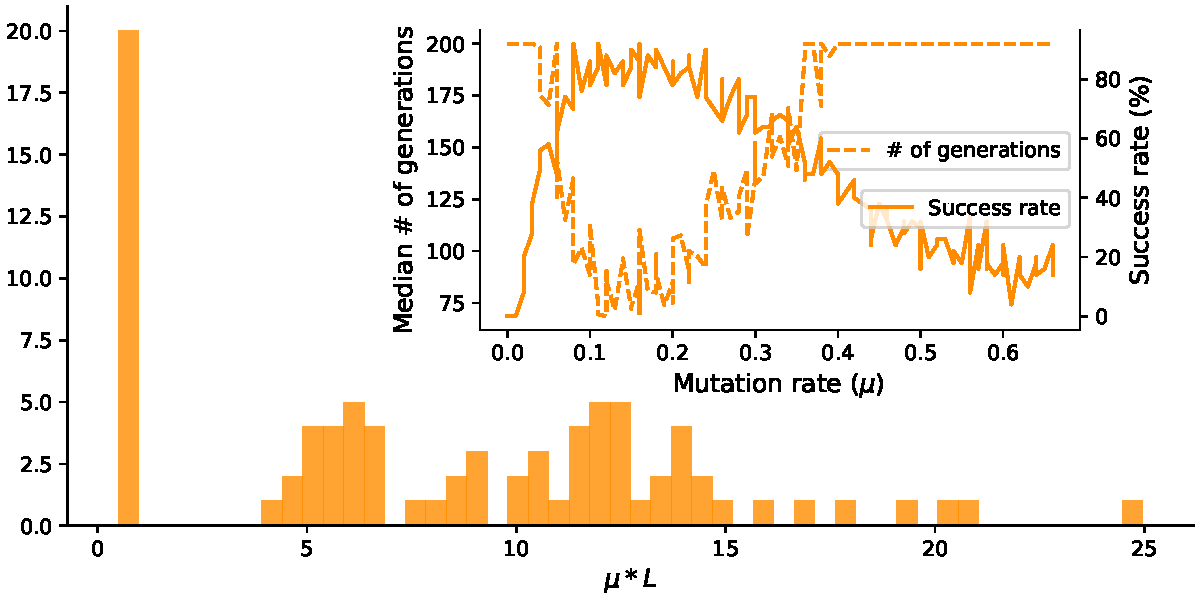
\includegraphics[width=1.0\linewidth]{figures/bino_tuning.pdf}
	%\caption{Binomial parameter tuning. Histogram of best mutation rate ($\mu^*$) for the same set of $81$ target structures with different pseudoknots and various lengths. The most frequent best parameter is the low mutation rate ($\approx 1/L$). For some structures, the mutation rate seems to be the high one for different lengths as well. Similar to the Levy mutation, The inset figure shows the median generations and the percentage of success \emph{vs.} the mutation rate ($\mu$) for one of the pseudoknotted target of length $88$ with a broader range of $\mu$ (from $0$ to $1$ with a step size of $1/L$)}\label{Fig:bino}
	%\medskip
	%\small.
	%\end{figure}
	\item Lévy mutation: we used the same dataset to tune the Zipf exponent $c$. First, for each $c \in [0,7]$ with a step size of $0.1$ and the same pseudoknotted target structure \texttt{PKB00342}, $100$ sequences were designed using \texttt{aRNAque}. The inset of Figure \ref{Fig:tunning}A shows the median number of generations and the success rate for each exponent $c$ respectively. The Zipf exponent distribution that produced the highest success rate and the minimum number of generations is $c*=1.4$. Secondly, for the $c \in [1,2]$ and a step size of $0.1$, an optimum exponent parameter $c*$ was investigated for all the $80$ remaining target structures. Figure \ref{Fig:tunning}A shows the histogram of $c*$. Contrary to binomial mutation, the optimum exponent parameter does not vary too much ($\forall \sigma$, $c*\approx 1$).  
\end{itemize}

\begin{figure*}[t!]
	\centering
	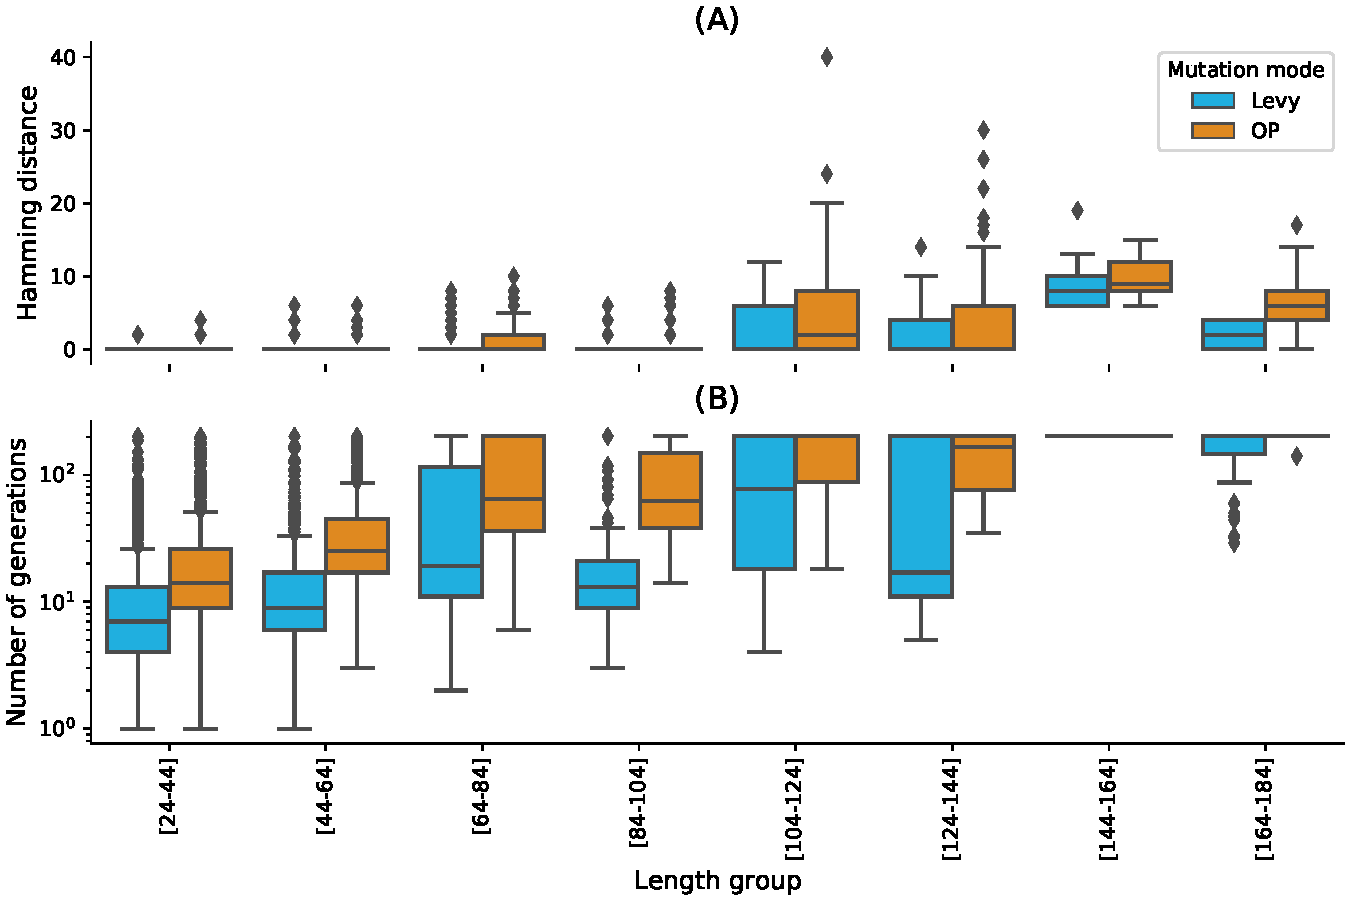
\includegraphics[width=1. \linewidth]{../res/images/arnaque/pkbase_ipknotV2.pdf}
	\caption{Lévy mutation mode \emph{vs} local mutation (one-point mutation). (A) Hamming distance distributions \emph{vs.} target structure lengths. (B)  Number of generations distributions for different length groups. In both (A) and (B), lower values indicate better performance. The target structures are solvable in less than $100$ generations for both mutation schemes and most length groups. Still, the difference in the number of generations gets more significant as the target lengths increase, except for the two last length groups for which both mutation schemes mostly failed. The highest difference in terms of median number of generations is $150$ for target lengths in the range $[124-144]$ (respectively $123, 49, 46, 16, 7, 0, 0$ for the length ranges $[84-104], [64-84], [104-124], [44-64], [24-44], [144-164], [164-184]$). Averaging over all length groups, the median number of generations difference between the Levy mutation and the one point mutation is $48$ generations. }\label{Fig:OP_vs_aRNAque}
	\medskip
	\small.
\end{figure*}
The main observation is that when using a Lévy mutation, the optimal mutation rate is approximately independent of the target structure. In contrast, the optimum binomial mutation rate parameter $\mu*$ varies with different targets. Although both mutation modes have approximately the same success rates ($88\%$ for the Lévy over $100$ runs and $\approx 92\%$ for the binomial over $50$ runs), the Lévy flight mutation scheme is more robust to different targets. Moreover, the median number of generations for the Lévy mutation is lower ($54$ for the Lévy and $92$ for the binomial mutation mode), thus enhancing efficiency.


\begin{figure*}[t!]
	\centering
	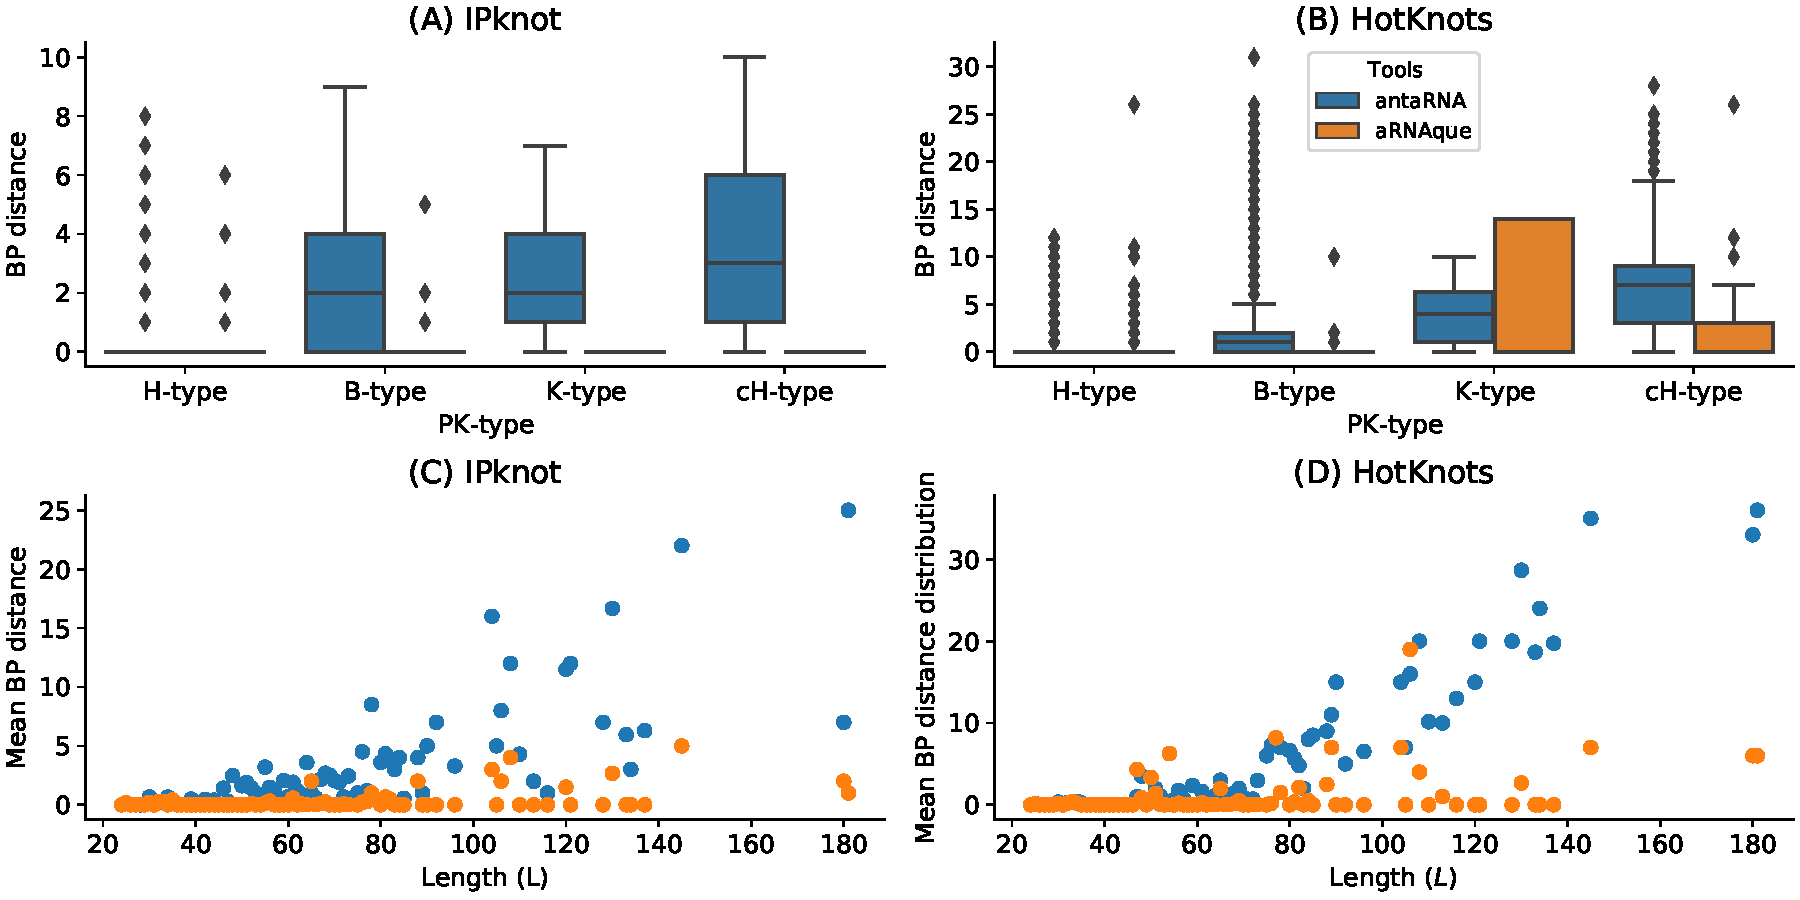
\includegraphics[width=1.0\linewidth]{../res/images/arnaque/pk_hotknot_IPknot_aRNAqueVSantaRNA_2.pdf}
	\caption{\texttt{aRNAque} \emph{vs} \texttt{antaRNA} on \texttt{PseudoBase++} dataset using both  \texttt{IPknot} and \texttt{HotKnots}. (A, B) Base pair distance distributions of the designed sequences to the target structure for different pseudoknot types. (C,D) Mean base pair distance against target lengths. }\label{Fig:antaRNA_vs_aRNAque}
	\medskip
	\small.
\end{figure*}

\section{Experimental results}
A Lévy mutation scheme offers a compromise between exploration at different scales (mostly local search combined with rare big jumps). Such a scheme significantly improves the number of evaluations needed to hit the target structure, while better avoiding getting trapped in local optima. We first compared the performance of \texttt{aRNAque} using Lévy mutations to the previous version with local mutations (binomial number of point-mutations with $\mu \approx \frac{1}{L}$). Secondly, we compared \texttt{aRNAque} to the existing pseudoknotted RNA inverse folding tool \texttt{antaRNA} using two folding tools: \texttt{HotKnots} and \texttt{IPknot}. We used the \texttt{PseudoBase++} dataset for both benchmarks. 


\subsection{Performance on \texttt{PseudoBase++}: Levy mutation \emph{vs.} Local mutation}
Figure \ref{Fig:OP_vs_aRNAque} shows box plots for the base pair distance (Hamming distance) and the number of generations for increasing target lengths under our two mutation schemes: binomial at low mutation rate (or one point mutation) and the Lévy mutation. For each pseudoknotted RNA target structure in the \texttt{PseudoBase++} dataset, we designed $20$ sequences.  The results show that using the Lévy mutation instead of a local mutation scheme can significantly increase the performance of \texttt{aRNAque}.  The gain was less significant in terms of designed sequences quality  (base pair distance distributions, with a $t$-value $\approx -1.04$ and $p$-value $\approx 0.16$) but more significant in terms of the average minimum number of generations needed for successful matches to target structures (with a $t$-value $\approx -3.6$ and $p$-value $\approx 0.0004$). This result demonstrates a substantial gain in computational time when using a Lévy mutation scheme instead of a purely local mutation.

\subsection{Performance on \texttt{PseudoBase++}: \texttt{aRNAque} \emph{vs.} \texttt{antaRNA}}

We also compared the sequences designed using \texttt{aRNAque} (with the Lévy mutation scheme) to those produced by \texttt{antaRNA}. Figures \ref{Fig:antaRNA_vs_aRNAque}A and \ref{Fig:antaRNA_vs_aRNAque}C show the base pair distance distribution for each category of pseudoknotted target structure and the mean of the base pair distance plotted against the length of the target secondary structures. For \texttt{antaRNA}, and when using \texttt{IPknot} as a folding tool, finding sequences that fold into the target becomes increasingly difficult with pseudoknot complexity (median base-pair distance distribution increases). On the other hand, \texttt{aRNAque}’s performance improves as pseudoknot complexity increases (e.g. the mean base-distance decreases with the pseudoknot complexity). In sum, as target length increases, the performance of \texttt{antaRNA} (local search) is considerably degraded , while \texttt{aRNAque} (Lévy flight search) stays almost constant.


%\begin{figure}[t!]
%\centering
%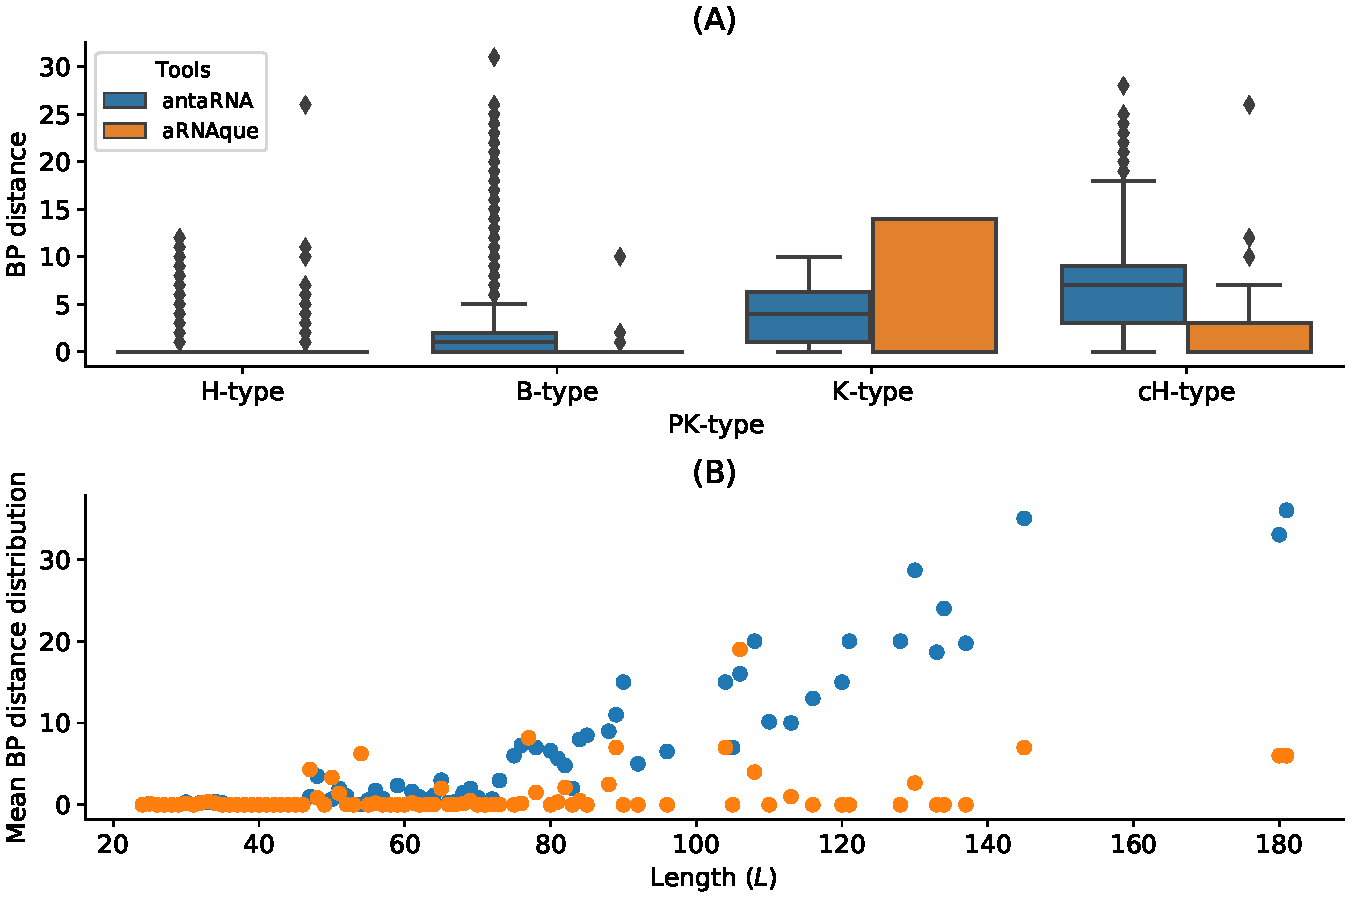
\includegraphics[width=1.0\linewidth]{figures/pk_hotknotaRNAqueVSantaRNA_2.pdf}
%\caption{\texttt{aRNAque} \emph{vs} \texttt{antaRNA} on \texttt{PseudoBase++} dataset using \texttt{HotKnots}. (A) Base pair distance distributions of the designed sequences to the target structure peer different pseudoknot types. (B) mean base pair distance against target lengths. }\label{Fig:antaRNA_hotknots}
%\medskip
%\small.
%\end{figure}
A second benchmark using \texttt{HotKnots} as a folding tool was performed on the same dataset. For both \texttt{aRNAque} and \texttt{antaRNA}, the more complex the pseudoknot motifs, the worse is the tool performance (median of the base-pair distance distribution increases). Figures \ref{Fig:antaRNA_vs_aRNAque}B and \ref{Fig:antaRNA_vs_aRNAque}D show the base pair distance distributions with respect to the pseudoknot motifs for both \texttt{aRNAque} and \texttt{antaRNA}. Even though both performances degrade as target length increases, \texttt{aRNAque} (Lévy flight evolutionary search) performance remains almost constant for all the target lengths greater than $60$.


\subsection{Performance on \texttt{Eterna100} dataset}

Finally, we performed a third benchmark on the \texttt{Eterna100} datasets. First, on the \texttt{Eterna100-V1} dataset, the Lévy flight version of \texttt{aRNAque} successfully designed $89\%$ of the targets and the one-point mutation (local mutation) version achieved $91\%$ of success. Combining the two datasets, \texttt{aRNAque} solved in total $92\%$ of the targets of \texttt{Eterna100-V1} (see also \cite{merleau2021simple}). When analysing the performance of Lévy flight for low and high base pair densities separately, the median number of generations of high base pair density targets was lower than the one with low base-pair density ($8$ generations for high density and $18$ for the low base pairs density targets). The same observation was drawn for the success rate. For the low base-pair density targets, the Lévy flight achieved $87\%$ ($49/56$) of success whereas, for the high base-pair density, it achieved $91\%$ ($40/44$). The same analysis can be done when comparing the one-point mutation results for the high-density targets to the Lévy flight mutation. The median number of generations for the low-density targets when using a one-point mutation operator was $34$ (respectively $24$ for the high base pair density targets) (see Figure \ref{Fig:diversity2}A). Second, a new benchmark was performed on \texttt{Eterna100-V2} with \texttt{aRNAque} achieving a $93\%$ success rate. Compared to recently reported benchmark results \cite{Eterna}, \texttt{aRNAque} achieved the similar performance to \texttt{NEMO} on \texttt{Eterna-V2}: one target was unsolved by all existing tools and one target solved only by \texttt{NEMO} remained unsolved by \texttt{aRNAque}. 


%\begin{table}[H]
%\centering
%\begin{tabular}{|c|c|c|}
%\hline
%& \texttt{aRNAque-v1}& \texttt{aRNAque-v2}\\
%\hline
%\texttt{Eterna100-V1}&  $91\%$ & $89\%$\\
%\hline
%\texttt{Eterna100-V2}&  $90\%$ & $94\%$\\
%\hline
%\end{tabular}
%\caption{Caption}
%\label{tab:my_label}
%\end{table}

\section{Conclusion}

In this work, we provide an updated version of \texttt{aRNAque} implementing a Lévy flight mutation scheme that supports pseudoknottted RNA secondary structures. The benefit of a Lévy flight over a purely local (binomial with $\mu<<1$ or a single point mutation) mutation search allowed us to explore RNA sequence space at all scales. Such a heavy tailed distribution in the number of point mutations permitted the design of more diversified sequences and reduced the number of evaluations of the evolutionary algorithm implemented in \texttt{aRNAque}. The main advantage of using a Lévy flight over local search is a reduction in the number of generations required to reach a target. This is because the infrequent occurrence of a high number of mutations allow a diverse set of sequences among early generations, without the loss of robust local search. One consequence is a rapid increase in the population mean fitness over time and a rapid convergence to the target of the maximally fit sequence. To illustrate that advantage, we ran \texttt{aRNAque} starting from an initial population of unfolded sequences both for a "one point mutation" and "Lévy mutation".

Figures  \ref{Fig:diversity}C and  \ref{Fig:diversity}D show respectively the max/mean fitness over time and the number of distinct structures discovered over time plotted against the number of distinct sequences. When using a Lévy mutation scheme, the mean fitness increases faster in the beginning but stays lower than the one using local mutations. Later in the optimisation, a big jump or high mutation on the RNA sequences produces structures with fewer similarities and, by consequence, worse fitness. In the $(5-10)^{th}$ generation, sequences folding into the target are already present in the Lévy flight population, but only at the $30^{th}$ generation are similar sequences present in the local search population. The Lévy flight also allows exploration of both the structure and sequence spaces, providing a higher diversity of structures for any given set of sequences (Figure \ref{Fig:diversity}D). Using the mean entropy of structures as an alternate measure of diversity, we see in Figure \ref{Fig:diversity}A how a Lévy flight achieves high diversity early in implementation, and maintains a higher diversity over all generations than a local search algorithm. Although the mutation parameters $P_C$ and $P_N$ influence the absolute diversity of the designed sequences, the Lévy flight always tends to achieve a higher relative diversity than local search, all else being equal. 

\begin{figure}[b!]
	\centering
	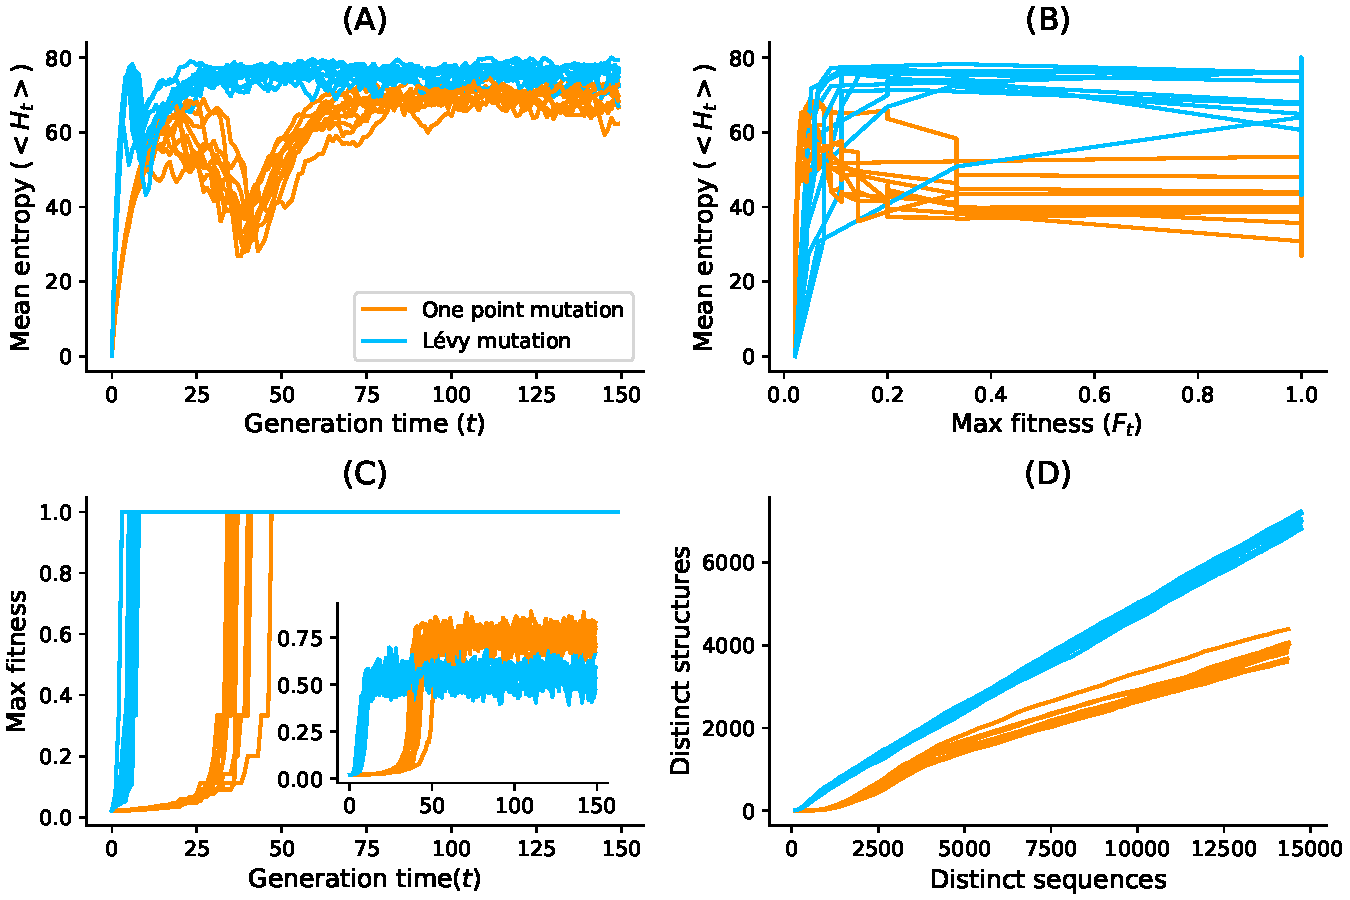
\includegraphics[width=1.0\linewidth]{../res/images/arnaque/diversity.pdf}
	\small
	\caption{Lévy mutation \emph{vs} one-point mutation: diversity analysis. For the \texttt{Eterna100} target structure \textit{[CloudBeta] 5 Adjacent Stack Multi-Branch Loop}, ten independent runs were performed in which a minimum of $10$ sequences were designed per run.  (A) Mean Shannon entropy of the population sequences over time for both binomial and Lévy mutation. (B) The max fitness plotted against the entropy over time. (C) Max fitness and mean fitness (inset) over time. (D) Distinct sequences \emph{vs.} Distinct structures over time.}
	\label{Fig:diversity}
	
\end{figure}
%The main advantage of using a Lévy mutation instead of a pure local mutation is more visible in the number of generations because high mutations allow earlier generations to generate compatible sequences---the sequences can be fitter depending on the initial population sequences. One consequence is the faster increase in the population mean fitness over time and the quicker convergence when looking at the max fitness. To illustrate that advantage, we ran \texttt{aRNAque} starting from an initial population of unfolded sequences both for a "one point mutation" and "Lévy mutation".  Figure \ref{Fig:diversity}C and \ref{Fig:diversity}D  show respectively the max/mean fitness over time and the number of distinct structures discovered over time plotted against the number of distinct sequences. Using a Lévy mutation scheme, the mean fitness increases faster in the beginning but stays lower than the one using local mutations. Later in the optimisation, a big jump or high mutation on the RNA sequences produces structures with fewer similarities and, by consequence, worse fitness.  In the early $25^{th}$ generation, sequences folding into the target are already in the population in the Lévy mutation case, wherein the local mutation case it's only at the $50^{th}$ generation. The Lévy flight allows also a better exploration of both the structure and the sequence spaces (Figure \ref{Fig:diversity}D). Thus, the designed sequences have high diversity (See Figure \ref{Fig:diversity}A). Although the mutation parameters $P_C$ and $P_N$ have a strong influence on the diversity of the designed sequences, when considering that the base pairs and nucleotides are selected uniformly during the mutations, the average population entropy of the RNA sequences using Lévy mutation tends to be higher than the one-point mutation one (Figure \ref{Fig:diversity}A).

%For the performance on the pseudoknotted RNA dataset, we first argue that the overall better performance of a Lévy mutation is due to the high base pairs density of the target RNA secondary structure. The more base pairs a target has; the faster the Levy mutation scheme is. To illustrate this, we clustered the benchmark datasets into two classes: one cluster for the target structures with a low base pair density (with density $\leq 0.5$) and a second cluster for the structure with high base pair density (with density $>0.5$). Figure \ref{Fig:diversity2}B shows the percentage of targets (for the \texttt{Eterna100} and the \texttt{PseudoBase++} dataset) with the low (respectively high) base pair densities. $71\%$ of the pseudoknotted target structures have a high base pair density which may explain why the Lévy mutation contributed to reducing the number of evaluations needed by \texttt{aRNAque} to hit the target. In contrast, the \texttt{Eterna100} dataset has almost equal targets with low and high base pair density. Analysing the performance of Lévy flight for the low and high base pair densities separately, the median number of generations of high base pair density targets was lower than the one with low base-pair density ($8$ generations for high density and $18$ for the low base pairs density targets). The same observation was drawn for the success rate. For the low base-pair density targets, the Lévy mutation achieved $87\%$ ($49/56$) of success, whereas for the high base-pair density, it achieved $91\%$ ($40/44$). The same analysis can be done when comparing the one-point mutation results for the high-density targets to the Lévy mutation. The median number of generations for the low-density targets when using a one-point mutation operator was $34$ (respectively $24$ for the high base pair density targets) (see Figure \ref{Fig:diversity2}A). We should also emphasise that the Lévy flight performance compared to \texttt{antaRNA} is partially influenced by the limitations of the folding tools---this may also explain the degradation of the inverse folding tools as the pseudoknot patterns get more complex.

We argue that the improved performance of the Lévy Flight over local search in target RNA structures is due to the high base pair density of pseudoknotted structures. Given that pseudoknots present a high density of interactions, there are dramatic increases in possible incorrect folds and thus becoming trapped near local optima \cite{hajdin2013accurate}. Large numbers of mutations in paired positions, as implied by a heavy tailed distribution, are necessary to explore radically different solutions. 

To illustrate that Lévy Flight performance was due to base pair density, we clustered the benchmark datasets into two classes: one cluster for target structures with low base pair density (density $\leq 0.5$) and a second cluster for structures with high base pair density (density $> 0.5$). Figure \ref{Fig:diversity2}B shows the number of target sequences available in each low and high density category. The number of targets available in each category are colored according to the percentage of pseudoknot-free targets (\texttt{Eterna100-V1}) vs. targets with pseudoknots (\texttt{Pseudobase++}), showing that pseudoknots are strongly associated with high base pair densities: $71\%$ of the pseudoknotted target structures have a high base pair density.  In contrast, the \texttt{Eterna100} dataset without psuedoknots has somewhat higher representation at low base pair density. If it is true that improved Lévy Flight performance is indeed tied to base pair density, it is possible that similar heavy-tailed mutation schemes could offer a scalable solution to even more complex inverse folding problems. 

\section*{Conclusion}
Although we believe that Lévy flight-type search algorithms offer a valuable alternative to local search, we emphasise that its enhanced performance over say \texttt{antaRNA} is partially influenced by the specific capabilities of existing folding tools. Their limitations may account for the degradation of these tools as the pseudoknot motifs get increasingly complex. Another possible limitation is that most pseudoknotted and pseudoknot-free target structures are relatively easy to solve (in less than $100$ generation time), requiring more investigations for the unsolved targets to illustrate the performance of the Lévy mutation better.



\begin{figure}[t!]
	\centering
	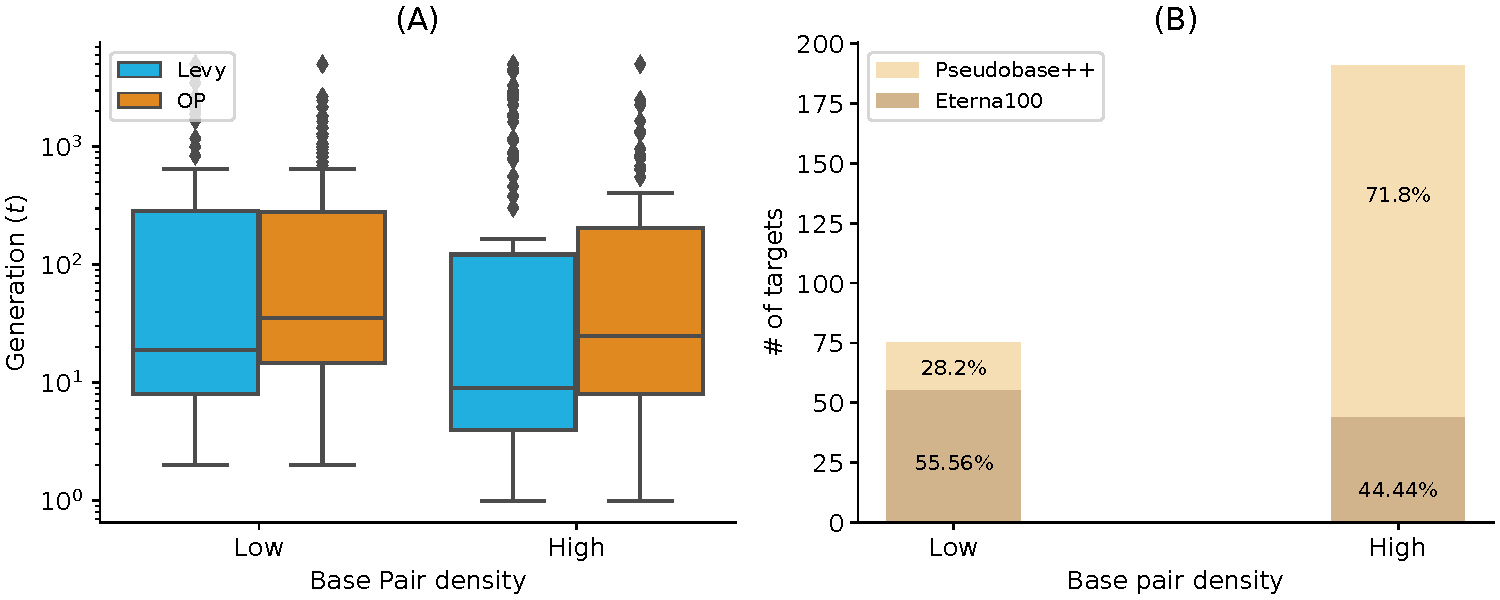
\includegraphics[width=1.05\linewidth]{../res/images/arnaque/levy_analysis.pdf}
	\small
	\caption{Lévy mutation \emph{vs.} one-point mutation: performance analysis with respect to the base-pair density. The higher the base-pair density is, the more useful the Lévy mutation scheme to speed up the optimization EA. (A) Distributions of number of generations for the low and high base-pair density targets of the \texttt{Eterna100} dataset. (B) Percentages of targets with low and high base-pair density for the \texttt{Eterna100} and \texttt{PseudBase++}}\label{Fig:diversity2}
\end{figure}

Our results show general and significant improvements in the design of RNA secondary structures compared to the standard evolutionary algorithm mutation scheme with a mutation parameter $\approx 1/L$, where $L$ is the sequence solution length. Not only does Lévy flight mutations lead to greater diversity of RNA sequence solutions, but it also reduces the evolutionary algorithm’s number of evaluations, thus improving computing time. 

%\textcolor{red}{
% Our results allow us to draw similar conclusions as in the earlier works %\cite{LevyGP,sharma2015modified}, which may open doors to a new standard or %default mutation scheme for an optimum evolutionary algorithm setting.
%}
\section*{Availability}
The implementation in \texttt{python3.7} of \texttt{aRNAque} and the benchmark data used in this manuscript are available at \url{https://github.com/strevol-mpi-mis/aRNAque}. We also provide the scripts used for the figures and the designed sequences analysis.
\section*{Competing interests}
The authors declare that they have no competing interests.

\section*{Author's contributions}
Text for this section \ldots

\section*{Acknowledgements}
We thank the Structure of Evolution Group at the Max Planck Institute for Mathematics in the Sciences, and especially Vincent Messow, for useful discussions. The Alexander von Humboldt Foundation provided funding for this work in the framework of the Sofja Kovalevskaja Award endowed by the German Federal Ministry of Education.